\documentclass[10pt,aspectratio=169]{beamer}

\usetheme{Madrid}
\usecolortheme{seahorse}
\useinnertheme{rectangles}
\useoutertheme{miniframes}

\usepackage[utf8]{inputenc}
\usepackage{graphicx}
\graphicspath{{ADEPT/data/models/tcn/}}
\usepackage{booktabs}
\usepackage{xcolor}
\usepackage{tikz}
\usepackage{array}
\usepackage{colortbl}

\definecolor{good}{RGB}{34,139,34}
\definecolor{warn}{RGB}{200,140,0}
\definecolor{bad}{RGB}{180,40,40}

\newcommand{\good}[1]{\textcolor{good}{\textbf{#1}}}
\newcommand{\warn}[1]{\textcolor{warn}{\textbf{#1}}}
\newcommand{\bad}[1]{\textcolor{bad}{\textbf{#1}}}

\title[ADEPT --- TCN Results]{ADEPT --- TCN Base Learner}
\subtitle{Phase 3 Results: Analysis and Next Steps}
\author{Guilherme Leit\~ao}
\institute[IST/INESC-ID]{Master Thesis --- IST / INESC-ID}
\date{\today}

\begin{document}

% ============================================================
\begin{frame}
  \titlepage
\end{frame}

% ============================================================
\begin{frame}{What was trained}
\begin{itemize}
  \item \textbf{Task:} same binary classification setting as RF Phase~2 ---
        same 4-attack dataset, same flow-level 70/15/15 split (seed=42),
        same adversarial exclusions (fuzzing / portscan / syn\_dos).
  \item \textbf{Input:} \texttt{sequence.npy} per source --- each sample is a
        $[T{=}10,\;F{=}1090]$ window (1\,088 nPrint header bits + IPAT z-score
        + Direction). Lazy-loaded via memmaps; $\sim$17\,GB per source.
  \item \textbf{Architecture:} 3-block causal TCN, channels $[128,128,128]$,
        kernel~3, dilations $\{1,2,4\}$, receptive field~29 $\gg T$,
        head: mean+max pooling $\to$ linear.
        \textbf{806\,018 parameters.} AMP enabled (CUDA).
  \item \textbf{Training:} AdamW ($\eta{=}10^{-3}$, wd$=10^{-4}$), cosine LR,
        \texttt{class\_weight=balanced}, early stopping patience~3 on
        val macro-F1.
\end{itemize}

\begin{block}{Headline metrics (test, overall)}
\centering
\begin{tabular}{lcccc}
\toprule
\textbf{Macro F1} & \textbf{ROC AUC} & \textbf{PR AUC} & \textbf{Recall (adv)} & \textbf{Precision (adv)} \\
\midrule
\warn{0.913} & \warn{0.974} & 0.985 & 0.854 & \good{0.999} \\
\bottomrule
\end{tabular}
\end{block}
\end{frame}

% ============================================================
\begin{frame}{Training behaviour}
\begin{columns}[T]
\column{0.55\linewidth}
\centering
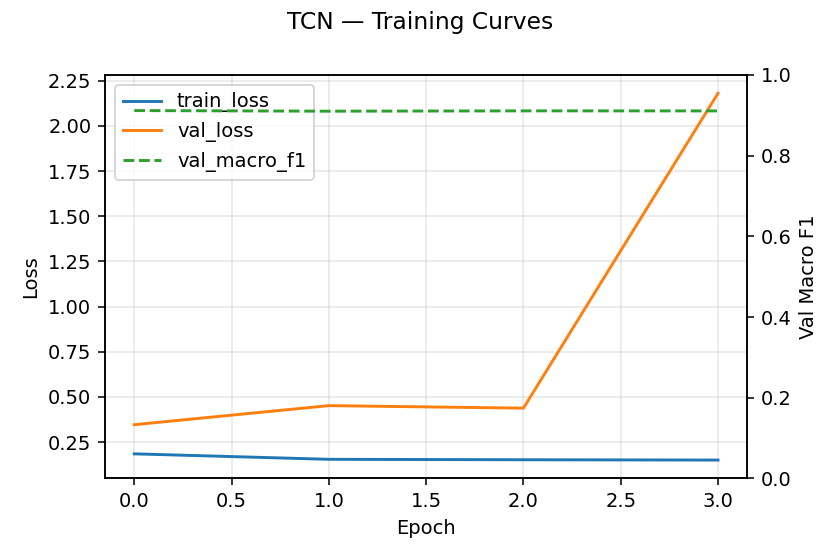
\includegraphics[width=\linewidth,height=0.72\textheight,keepaspectratio]{training_curves.png}

\column{0.45\linewidth}
\small
\begin{tabular}{cccc}
\toprule
\textbf{Ep.} & \textbf{Tr.\ loss} & \textbf{Val.\ loss} & \textbf{Val.\ F1} \\
\midrule
0 & 0.185 & 0.347 & \good{0.912} \\
1 & 0.155 & 0.452 & 0.910 \\
2 & 0.153 & 0.438 & 0.911 \\
3 & 0.151 & \bad{2.181} & 0.911 \\
\bottomrule
\end{tabular}

\vspace{0.5em}
\begin{itemize}\scriptsize
  \item \textbf{Best checkpoint: epoch~0} (first pass through data).
        Val macro-F1 never improved thereafter.
  \item Train loss decreases while val loss climbs --- early
        overfitting.  Val-loss spike at epoch~3 is consistent with
        AMP overconfidence: class probabilities approach 0/1,
        driving log-loss up while argmax F1 stays flat.
  \item Early stopping (patience=3) triggered correctly; saved
        checkpoint is unaffected.
\end{itemize}
\end{columns}
\end{frame}

% ============================================================
\begin{frame}{Confusion matrix \& curves}
\begin{columns}[t]
\column{0.33\linewidth}
\centering
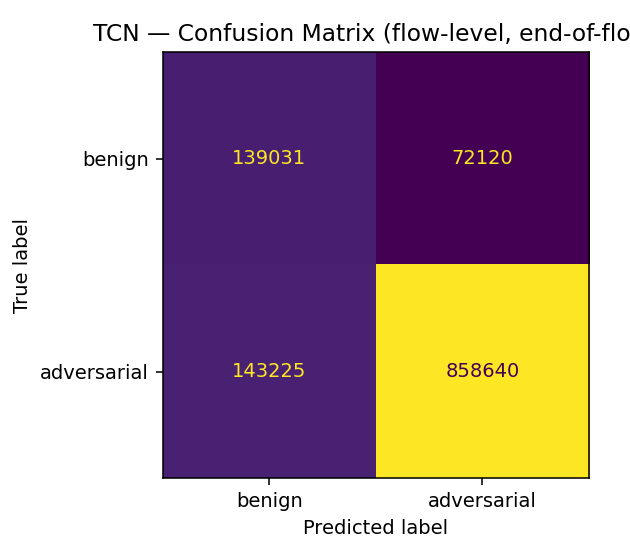
\includegraphics[width=\linewidth]{confusion_matrix.png}\\[2pt]
{\scriptsize Confusion Matrix}

\column{0.33\linewidth}
\centering
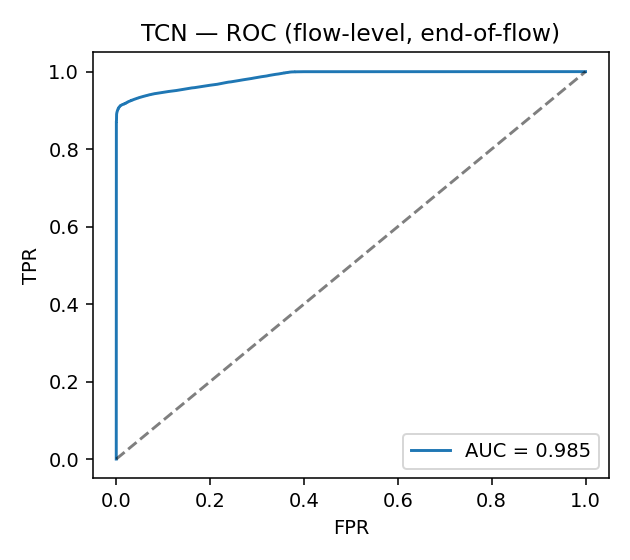
\includegraphics[width=\linewidth]{roc_curve.png}\\[2pt]
{\scriptsize ROC (AUC = 0.974)}

\column{0.33\linewidth}
\centering
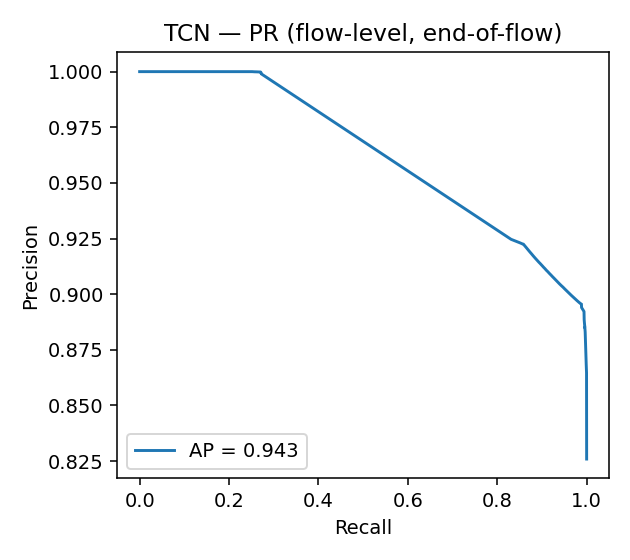
\includegraphics[width=\linewidth]{pr_curve.png}\\[2pt]
{\scriptsize Precision--Recall (AP = 0.985)}
\end{columns}

\vspace{0.5em}
\begin{itemize}\small
  \item High adversarial \emph{precision} (0.999): when the TCN fires, it is
        almost never wrong --- very few false positives.
  \item Moderate adversarial \emph{recall} (0.854): 14.6\% of adversarial
        windows are missed --- mainly IAT-only and Mirai variants (see next
        slides).
\end{itemize}
\end{frame}

% ============================================================
\begin{frame}{Per-variant performance (vs.\ balanced benign)}
\centering\small
\begin{tabular}{lccc}
\toprule
\textbf{Variant} & \textbf{F1$_\text{adv}$} & \textbf{ROC AUC} & \textbf{PR AUC} \\
\midrule
\rowcolor{good!15} ddos\_adv\_both / size       & 0.994 / 0.992 & 1.000 / 0.999 & 1.000 / 0.998 \\
\rowcolor{warn!15} ddos\_adv\_iat               & \warn{0.401} & 0.956 & \warn{0.697} \\
\midrule
\rowcolor{good!15} dos\_slow\_adv\_both / size   & 0.997 / 0.997 & 1.000 & 1.000 \\
\rowcolor{warn!15} dos\_slow\_adv\_iat           & \warn{0.797} & 0.960 & \warn{0.880} \\
\midrule
\rowcolor{good!15} ssdp\_flood\_adv\_\{both, iat, size\} & 0.995 / 0.993 / 0.995 & 1.000--0.9997 & 1.000--0.999 \\
\midrule
\rowcolor{warn!15} mirai\_adv\_both / size      & 0.376 / 0.473 & 0.587 / 0.627 & 0.324 / 0.405 \\
\rowcolor{bad!15}  mirai\_adv\_iat              & \bad{0.000}   & 0.562 & \bad{0.110} \\
\bottomrule
\end{tabular}

\vspace{0.5em}
\begin{itemize}\small
  \item \good{SSDP Flood:} near-perfect across all modes --- header patterns
        uniquely identify TANTGen perturbations.
  \item \warn{DDoS / DoS Slow IAT:} recall collapses when only timing
        is perturbed --- the single IPAT z-score is drowned by
        1\,088 unchanged header bits.
  \item \bad{Mirai:} low F1 across all modes; IAT variant is a
        complete failure (0 adversarial predictions out of 2\,928).
\end{itemize}
\end{frame}

% ============================================================
\begin{frame}{Same-base vs.\ balanced benign: where detection is harder}
\centering\small
\begin{tabular}{lcc>{\columncolor{warn!10}}c}
\toprule
\textbf{Variant} & \textbf{F1 (balanced)} & \textbf{F1 (same-base)} & \textbf{$\Delta$} \\
\midrule
\rowcolor{good!15} ddos\_adv\_both / size        & 0.994 / 0.992 & 1.000 / 0.998 & $+$0.003--$+$0.006 \\
\rowcolor{warn!15} ddos\_adv\_iat                & 0.401 & 0.405 & $+$0.004 \\
\rowcolor{good!15} dos\_slow\_adv\_both / size   & 0.997 / 0.997 & 0.999 / 0.999 & $+$0.001--$+$0.002 \\
\rowcolor{warn!15} dos\_slow\_adv\_iat           & 0.797 & 0.799 & $+$0.002 \\
\rowcolor{good!15} ssdp\_flood\_adv\_\{both, iat, size\} & 0.995--0.997 & 0.997 & $\approx$\,0 \\
\rowcolor{warn!15} mirai\_adv\_both / size       & 0.376 / 0.473 & 0.380 / 0.476 & $\approx$\,0 \\
\rowcolor{bad!15}  mirai\_adv\_iat               & 0.000 & 0.000 & 0 \\
\bottomrule
\end{tabular}

\vspace{0.4em}
\begin{itemize}\small
  \item \good{Volumetric attacks:} same-base F1 $\geq$ balanced F1 --- TANTGen's
        payload / IPAT shifts are prominent even against same-source benign.
  \item \warn{Mirai / IAT variants:} unlike the RF, the TCN does \emph{not}
        show same-base bleed; F1 is uniformly weak regardless of benign pool
        --- the TCN simply cannot discriminate these variants, independent
        of benign mix.
\end{itemize}
\end{frame}

% ============================================================
\begin{frame}{RF vs.\ TCN: head-to-head (F1$_\text{adv}$, balanced benign)}
\centering\small
\begin{tabular}{lccc}
\toprule
\textbf{Variant} & \textbf{RF} & \textbf{TCN} & \textbf{Winner} \\
\midrule
ddos\_adv\_both / size   & 0.91 / 0.91 & \good{0.994 / 0.992} & \good{TCN (+0.08)} \\
ddos\_adv\_iat           & \good{0.90} & 0.401 & \good{RF (+0.50)} \\
dos\_slow\_adv\_both / size & 0.955 / 0.955 & \good{0.997 / 0.997} & \good{TCN (+0.04)} \\
dos\_slow\_adv\_iat      & \good{0.953} & 0.797 & \good{RF (+0.16)} \\
ssdp\_flood\_adv\_both / iat / size & 0.91 & \good{0.993--0.995} & \good{TCN (+0.08)} \\
mirai\_adv\_both / iat / size & \good{0.887 / 0.883 / 0.761} & 0.376 / 0.000 / 0.473 & \good{RF (+0.3--0.9)} \\
\bottomrule
\end{tabular}

\vspace{0.5em}
\begin{itemize}\small
  \item \good{TCN dominates on size/both modes} --- nPrint header bits encode
        payload padding directly; 3 blocks of causal convolutions detect
        TANTGen's structural changes better than RF aggregates.
  \item \good{RF dominates on IAT-only modes and Mirai} --- aggregated
        IPAT statistics (mean/std/min/max) give IAT a 16.7\% feature share;
        the TCN's single IPAT z-score at 0.09\% is swamped.
  \item \textbf{The two models are complementary} --- the meta-learner
        can route by perturbation mode.
\end{itemize}
\end{frame}

% ============================================================
\begin{frame}{Why IAT modes fail: feature geometry}
\begin{columns}[T]
\column{0.5\linewidth}
\textbf{TCN input: 1\,090 features per packet}
\begin{itemize}\small
  \item 1\,088 nPrint header bits (IP flags, TTL, ports, TCP flags,
        payload size bytes, \ldots)
  \item 1 IPAT z-score (\emph{the only IAT signal})
  \item 1 Direction bit
\end{itemize}

\vspace{0.4em}
IPAT share = $1 / 1090 \approx \mathbf{0.09\%}$

\vspace{0.4em}
\textbf{RF input: 24 aggregate features per window}
\begin{itemize}\small
  \item 4 IPAT statistics: mean, std, min, max
  \item 20 other aggregates (packet size, payload, TCP flags, \ldots)
\end{itemize}

IPAT share = $4 / 24 \approx \mathbf{16.7\%}$

\column{0.5\linewidth}
\textbf{Consequence}

\vspace{0.4em}\small
IAT-only perturbations change exactly 1 out of 1\,090 features per
packet. The convolutional filters learn to rely on the 1\,088
unchanged header bits (which strongly identify the traffic type),
rendering the IPAT z-score invisible.

\vspace{0.5em}
This also explains the Mirai IAT complete failure (0 detections):
Mirai headers are particularly uniform within a capture, so the TCN
confidently predicts \emph{benign} for every window --- it never sees
enough contrast in the header bits to trigger on the timing signal.

\vspace{0.5em}
\textbf{Fix candidates for future work:}
\begin{itemize}\scriptsize
  \item Drop nPrint bits; use IPAT-only sequence (matches RF's focus).
  \item Feature groups with separate convolution streams.
  \item Add explicit IPAT features at multiple lags.
\end{itemize}
\end{columns}
\end{frame}

% ============================================================
\begin{frame}{Conclusions}
\begin{enumerate}
  \item \good{SSDP Flood and DoS Slow (both/size modes) are detected
        near-perfectly (F1$_\text{adv}$ $\geq$ 0.993)} --- causal
        convolutions over nPrint sequences capture payload-level TANTGen
        perturbations better than RF aggregates.
  \item \good{TCN outperforms RF on all size/both modes by 4--8 F1
        points} --- structural header changes are directly visible in the
        raw packet sequence.
  \item \warn{IAT-only modes are the TCN's Achilles heel} --- IPAT
        accounts for 0.09\% of the input; the model ignores it.
        DDoS IAT F1 drops to 0.401; DoS Slow IAT to 0.797.
  \item \bad{Mirai is entirely missed}: F1$_\text{adv}$ 0.37--0.47
        for both/size, \bad{0.000} for IAT --- the most critical
        limitation of this run.
  \item \warn{Training converged in a single epoch} (best\_epoch=0);
        the val-loss spike at epoch~3 is consistent with AMP
        overconfidence but does not affect the saved checkpoint.
  \item \good{RF and TCN are strongly complementary} --- their
        weak spots are disjoint, motivating the meta-learner fusion
        in Phase~4.
\end{enumerate}
\end{frame}

% ============================================================
\begin{frame}{Next steps}
\textbf{Short-term (End of May) --- complete the ensemble \& tune end-to-end}
\begin{enumerate}\scriptsize
  \item \textbf{Phase 4 --- Mini-Transformer meta-learner} fusing RF + TCN logits via
        self-attention. Expected to recover Mirai / IAT variants where
        RF is stronger.
  \item \textbf{TCN feature investigation} --- ablation: IPAT-only sequence vs.\ full
        nPrint. If IPAT-only closes the Mirai gap, feed it as a separate stream.
  \item \textbf{Sync with In\^es} on TANTGen version in use ---
        confirm Fuzzing snaplen-200B no-op and whether Mirai IAT
        perturbation magnitude is configurable.
  \item \textbf{DPSS hyperparameter sweep} --- grid-search
        \texttt{window\_size} $\in \{5,10,20\}$, TCN channels/depth,
        meta-learner params. Objective: maximize ensemble detection
        accuracy.
\end{enumerate}

\textbf{Long-term --- defense layer \& write-up}
\begin{enumerate}\scriptsize\setcounter{enumi}{4}
  \item \textbf{Phase 5 --- Purification Transformer} (decoder-only Seq2Seq)
        projecting adversarial windows back onto the benign manifold;
        KV-caching for latency.
  \item \textbf{Phase 6 --- RL Adaptation Agent} re-weighting the ensemble
        online from TANTGen feedback + offline DPI validation.
  \item \textbf{Dissertation write-up.}
\end{enumerate}
\end{frame}

% ============================================================
\begin{frame}[fragile]{Reproducibility}
\textbf{Artifacts under} \texttt{ADEPT/data/models/tcn/}
\begin{itemize}\small
  \item \texttt{tcn.pt} --- best model state\_dict (epoch~0)
  \item \texttt{metrics.json} --- overall + per-source (vs\_all / vs\_balanced /
        vs\_same\_base) + per-\texttt{label\_str}
  \item \texttt{split.npz}, \texttt{dataset\_index.npz} --- exact train/val/test
        partition (shared with RF via \texttt{assemble\_index})
  \item \texttt{training\_info.json}, \texttt{training\_curves.json},
        \texttt{tcn\_config.json} --- full training trace and resolved config
  \item \texttt{*.png} --- confusion matrix, ROC, PR, training curves
\end{itemize}

\vspace{0.6em}
\textbf{Re-run from scratch}
\begin{block}{}
\small
\begin{verbatim}
python3 scripts/adversarial_generation/generate_adversarials.py
python3 scripts/packet_to_tensor/process_all_attacks.py --tantgen
python3 scripts/tcn/run_tcn.py
\end{verbatim}
\end{block}
\end{frame}

\end{document}
